
\documentclass[preprint,authoryear]{elsarticle}

\usepackage[utf8]{inputenc}
\usepackage{xcolor}
\usepackage{amsmath}

\newcommand{\memo}[2]{\textcolor{#1}{#2}}
\newcommand{\xavi}[1]{\memo{orange}{xavi: #1\\}}
\newcommand{\enrico}[1]{\memo{blue}{enrico: #1\\}}

\journal{Theoretical Population Biology}

\begin{document}

\begin{frontmatter}

\title{Allee Effect and Cultural Evolution}
%\title{The evolution of payoff-biased learning under Allee Effect} %Perhaps a 


\author[label1,label2]{Enrico R. Crema\corref{cor1}}
\cortext[cor1]{Corresponding Author: enrico.crema@upf.edu}
\author[label3]{Xavier Rubio-Campillo}

\address[label1]{CaSEs - Complexity and Socio-Ecological Dynamics Research Group, Barcelona}
\address[label2]{UCL Institute of Archaeology}
\address[label3]{BSC - Barcelona Supercomputing Center}



\begin{abstract}
Social learning rules are often guided by the amount of payoff received by potential social teachers while expressing specific cultural traits. The assumption of the social learner is that such payoff is a proxy for inferring the qualitative features of the target trait. Here we explore the theoretical implications when payoff directly affects  reproductive fitness and its expected amount is a function of the number of individuals possessing the given trait. More specifically we consider a particular form of density-dependence where a too small or too large population of individuals possessing the same variant will be subject to a decline in fitness, while an intermediate size is optimal. This non-linear relationship, known as Allee effect, portrays a large number of behavioural traits, in particular subsistence strategies that are enhanced  by the effect of cooperation but are constrained by interference and limited resources. We  explores the evolutionary dynamics of a single trait model  with two variants, each exhibiting a different Allee effect. We used a modified Lotka-Volterra model of payoff-biased social learning, and show that different degrees of reliance on social learning can exhibit a variety of equilibria, including episodes of reversion, stable co-existence, and fixation to one variant.

% XAVI: I'm confused by the use of trait and variant: shouldn't it be 'a single trait model with two variants'?
% I'm using them as synonym, but I guess you have a point. 

\end{abstract}

\begin{keyword}
Social Learning\sep Subsistence\sep Allee Effect\sep Cooperation\sep Carrying Capacity
\end{keyword}

\end{frontmatter}

\section{Introduction}



A central element of all social learning strategies is the presence of some heuristics that offers some guidance in the selection of a given variant over another. This  can be based on some properties of the variant itself (\emph{content-bias}) or derived from contextual cues (\emph{context-bias}), such as the commonness or the rareness of a trait, or some features associated with the transmitter such as prestige, success, or his/her similarity to the learner~\citep{henrich_mcelreath2003}. An expected consequence of \emph{context-bias} is the possibility of a feedback process, whereby the attractiveness of a given variant might change as a consequence of the learning strategy~\citep{kendal_etal_2009}. For example a strong anti-conformist bias might initially favour rare traits, but as they spread into a population their selective advantage will decline as the result of a negative feedback. On the other hand conformist-bias and homophily-guided learning strategies are expected to exercise a positive feedback to some form of fixation. 

This paper examines a group of learning strategies generally referred to as \emph{payoff-based transmission}~\citep{schlag1998,kendal_etal_2009,lake_and_crema_2012,baldini2013,kandler_and_laland_2013,crema_lake_inpress}. The core assumption shared by these models is that the probability of copying a given cultural trait $i$ is positively correlated with a payoff signal $s$, determined by some function $f(i)$ expressed by individuals possessing the trait itself. Several variants of this learning strategies have been proposed and explored, including: \emph{imitate the best}, where the social learner identifies and copies the trait possessed by the individual with the highest payoff; \emph{compare means}, where the social learner compare the average payoff of different strategies and chooses the highest variant; and the \emph{proportional imitation rule}, where the probability of adopting a variant is proportional to the difference in payoff between the demonstrator and the learner~\citep{schlag1998,baldini2013}. 

Whilst most studies focused on how the difference in these imitation rules can drive the dynamics of the system, less attention has been paid on the payoff signal.  The exact nature of the signal is most likely some indirect proxy that is assumed, by the social learner, to be linked with the target cultural trait. Thus one might be guided by a variety of cues (e.g. number of offpsring, income, presence/absence of other traits associated with success or prestige, etc.) that are differently correlated with the target trait resulting into different degrees of uncertainty in the signal. The magnitude of this uncertainty can have strong impact to efficiency of specific learning rules. For example,~\citet{crema_lake_inpress} have shown that \emph{imitate the best} is negatively correlated with payoff uncertainty. In the case of high uncertainty, a novel trait with payoff higher than the average has a decreased probability of being selected, due to being initially rare in a population. This can generate scenarios dominated by extant suboptimal variants.

Given the same cultural trait, the variability in the payoff signal is partly derived by the presence of interacting cultural and physical traits, as well as the environment where the trait is manifest. Thus the payoff is better described by the function $f(i,\epsilon)$, where $i$ is the trait, and $\epsilon$ is a series of additional hidden or latent variables that might or might interact with $i$. For example, a fisherman might evaluate the performance of a hook (the target cultural trait) using as a cue the number of fish captured (the payoff signal). The correlation between the two is partly due to the efficiency of the hook, but also by the rod, the choice of the bait, the availability of the prey species, the choice of the fishing spot, the physical properties of the fisherman, and chance. In many cases we should expect that the social teacher and learner share many of these interacting traits as well as the environment where these are displayed. In other words, cultural and ecological inheritance can generally reduce the impact of $\epsilon$, and consequently the uncertainty and the variability in the payoff-signal. There are however exceptions. One of these are contexts where the success of a variant is strongly correlated with the absolute number of individuals $n_i$ possessing the same trait within a population. This density dependence, which can be described by the payoff function $f(i,n_i)$, implies that the adoption (or abandonment) of a trait can alter the expected payoff-signal, possibly generating a variety of feedback mechanism.  

Several cultural traits are expected to show such density dependence. In particular, behaviour linked to the exploitation of limited resources are expected to exhibit a negative density dependence. Novel optimal variants are likely to spread rapidly when the trait is rare, but once a threshold frequency is exceeded (i.e. the carrying capacity),  beneficial effect will start to decline, the payoff will become smaller, and eventually rarer suboptimal variants can be preferred (see Lake and Crema 2012 for an extensive analysis). 

However, density dependence does not necessarily imply only a negative correlation between population size and payoff/fitness. In many ecological contexts an inverse density dependence, whereby per capita growth rate is positively correlated with population density, has been noted. This phenomena, known as Allee effect \citep{allee1958,courchamp_etal_1999}, is generally explained by a range of processes from cooperation to unconscious mutual facilitation that enhances individual fitness at low population density. This inverse density dependence can be further distinguished between \emph{weak} and \emph{strong} Allee effect. In the former case, the reproductive fitness is always positive at low population density, whilst in the latter case we expect the presence of a critical density below which fitness becomes negative \citep{Wang_and_Kot_2001}. 






Variants that are enhanced by some form of cooperation, or more in general traits exhibiting a positive niche construction are expected to show such a pattern, known in ecology as \emph{Allee Effect}~\citep{allee1958}. 

While a systematic review of the empirical evidence of Allee effect has been conducted in population ecology \citep{kramer_etal_2009}, no 

For example foraging groups are known to show higher performance when the number of individuals is not too small~\citep{hill_and_hawkes_1983,janssen_and_hill_2014}, while certain activities such as anthropogenic fire~\citep{bird2013} or selective hunting~\citep{dods_2002} might require a population density beyond a certain threshold in order to promote sufficient niche enhancement and a consequent increase in payoff~\citep{rowley-conwy_and_layton_2011}. Other traits that might be promoted by increased density includes language~\citep{kandler2009}, organisational populations~\citep{caroll_and_hannan_1989} and communication technologies~\citep{van_slyke_perceived_2007}.



%We definitely need to add some literature review on the theorethical models of Allee effect here as an additional paragraph.

Here we explore the combined effect of positive and negative density-dependent selection, assuming that: 1) the social learning strategy is payoff-based transmission; and 2)  payoff is equivalent to the reproductive fitness of each individual. We will demonstrate, by exploring a two-trait difference equation, that the impact of Allee effect on social learning can strongly affect the evolutionary trajectory of the system leading to the emergence of stable and unstable equilibria, as well as the occurrence of temporary or permanent episodes of reversion to suboptimal variants.


\section{The Model}
We consider the evolutionary dynamics of two mutually exclusive subsistence strategies whose fitness has both positive and negative density dependence. In particular we examine how two population of individuals, $a$ and $b$, change over time if we allow for a social learning strategy guided by a \emph{proportional imitation rule} (i.e. the probability of an individual with lower payoff to adopt the trait of an individual with higher payoff is proportional to the difference in the payoff). The model can theoretically be extended to $n$ strategies, but here we decide to explore a two trait version for simplicity. The core model can be depicted with the coupled difference equation \eqref{eq1}:

\begin{align}
\begin{cases}
a_{t+1}& = a_t + a_t R_{a,t} + C_{a,b,t} \\
b_{t+1}& = b_t + b_t R_{b,t} + C_{a,b,t}
\end{cases}
\label{eq1}
\end{align}

where $a_{t+1}$ and $b_{t+1}$ are the population using each trait at time $t+1$. This is given by the number of individuals during the previous time-step ($a_t$ and $b_t$), the reproductive rate of each population ($R_{a,t}$ and $R_{b,t}$), and the shift from one population to another dictated by cultural transmission ($C_{a,b,t}$).
% XAVI do you want to use cultural trasmission here or better stick with social learning?
The reproductive growth rate $R$ of each population is defined by the following paired equation:

\begin{align}
\begin{cases}
R_{a,t}& = r_a (\frac{a_t}{A_a}-1)(1-\frac{a_t}{K_a})\\
R_{b,t}& = r_b (\frac{b_t}{A_b}-1)(1-\frac{b_t}{K_b}) 
\end{cases}
\label{eq2}
\end{align}

where $r$ is the basic growth rate, $A$ is the \emph{Allee} threshold and $K$ is the carrying capacity, following the condition $A < K$. Equation \eqref{eq2} implies that the reproductive rate is negative when density is below $A$ or above $K$, and will reach its maxima $R_{max}=\frac{r(A-K)2}{4AK}$ when the population density is equal to $\frac{(K-A)}{2}$. 

Cultural transmission is portrayed in \eqref{eq3}:

\begin{align}
\label{eq3}
C_{a,b,t} = 
\begin{cases}
0& \text{if } R_{a,t} = R_{b,t}\\
\zeta(a_t+a_tR_{a,t})& \text{if } R_{a,t} > R_{b,t}\\
-\zeta(b_t+b_tR_{b,t})& \text{if } R_{a,t} < R_{b,t}
\end{cases}
\end{align}

where $\zeta$ defines the proportion of individuals changing strategy, and given by \eqref{eq4}:

\begin{align}
\label{eq4}
\zeta = 
\begin{cases}
z& \text{if }|R_{a,t}-R_{b,t}| > b\Delta\\
z\frac{|R_{a,t}-R{b,t}|}{m\Delta}& \text{if }|R_{a,t}-R_{b,t}| \leq b\Delta\\
\end{cases}
\end{align}

% XAVI b is not explained?
where $z$ is a measure of reliance in social learning (effectively equivalent to highest possible transmission rate), $\Delta$ is the maximum between $R_{max(a,t)}$ and $R_{max(b,t)}$, and $m$ is a calibration parameter that measure the perception of the difference in the payoffs (i.e. small values of $m$ determines a higher rate by which the theoretical maximum transmission rate is reached). Thus \eqref{eq3} and \eqref{eq4}  conforms with the \emph{proportional imitation rule}~\citep{schlag1998}, although here the payoff is equivalent to the reproduction rate. 

\section{Results}

We investigate the equilibrium conditions for different initial population sizes of  $a$ and $b$ and different settings of $z$, $A$, and $K$, assuming that  $r_a=r_b$, and for convenience holding the condition $K_b \geq K_a$. Given that equations \ref{eq1}-\ref{eq4} have no analytical solution, we identified equilibrium conditions via simulation (see appendix 1 for details; source code can be found on the following repository %put link here
as well as in the ESM).  
%if the points we need to reiterate are short, perhaps a footnote will suffice instead of an appendix? 
% 100,000 iterations 
% basin plots resolution

\subsection{Equilibrium conditions without social learning}

When $z=0$, equations \ref{eq1}-\ref{eq4} \emph{de facto} portray a standard cubic growth model with Allee effect, where the success (or failure) of a given focal trait is simply given by its own density, and the density of alternative cultural traits has no influence. For a generic cultural trait $x$, the model predicts three point attractors at $x=0$ (extinction), $x=A_x$, and $x=K_x$. The equilibrium $x=A_x$ is unstable in all cases, whereas the stability of the node at $x=K_x$ is a function of the per capita growth rate $r_x$. Increasing the latter decreases the stability of fixed points~\citep{scheuring_1999}, leading to the transition from point attractors (with equilibrium at $x=K_x$), to limit cycles and chaotic dynamics with islands of stability (see fig. \ref{fig:bifurcationDiagram}). % Not sure if there are strange attractors.  Reference  any  bifurcation analysis on the equation we used. Scheuring 1999 on JTB?

\begin{figure}[h!]
  \centering
      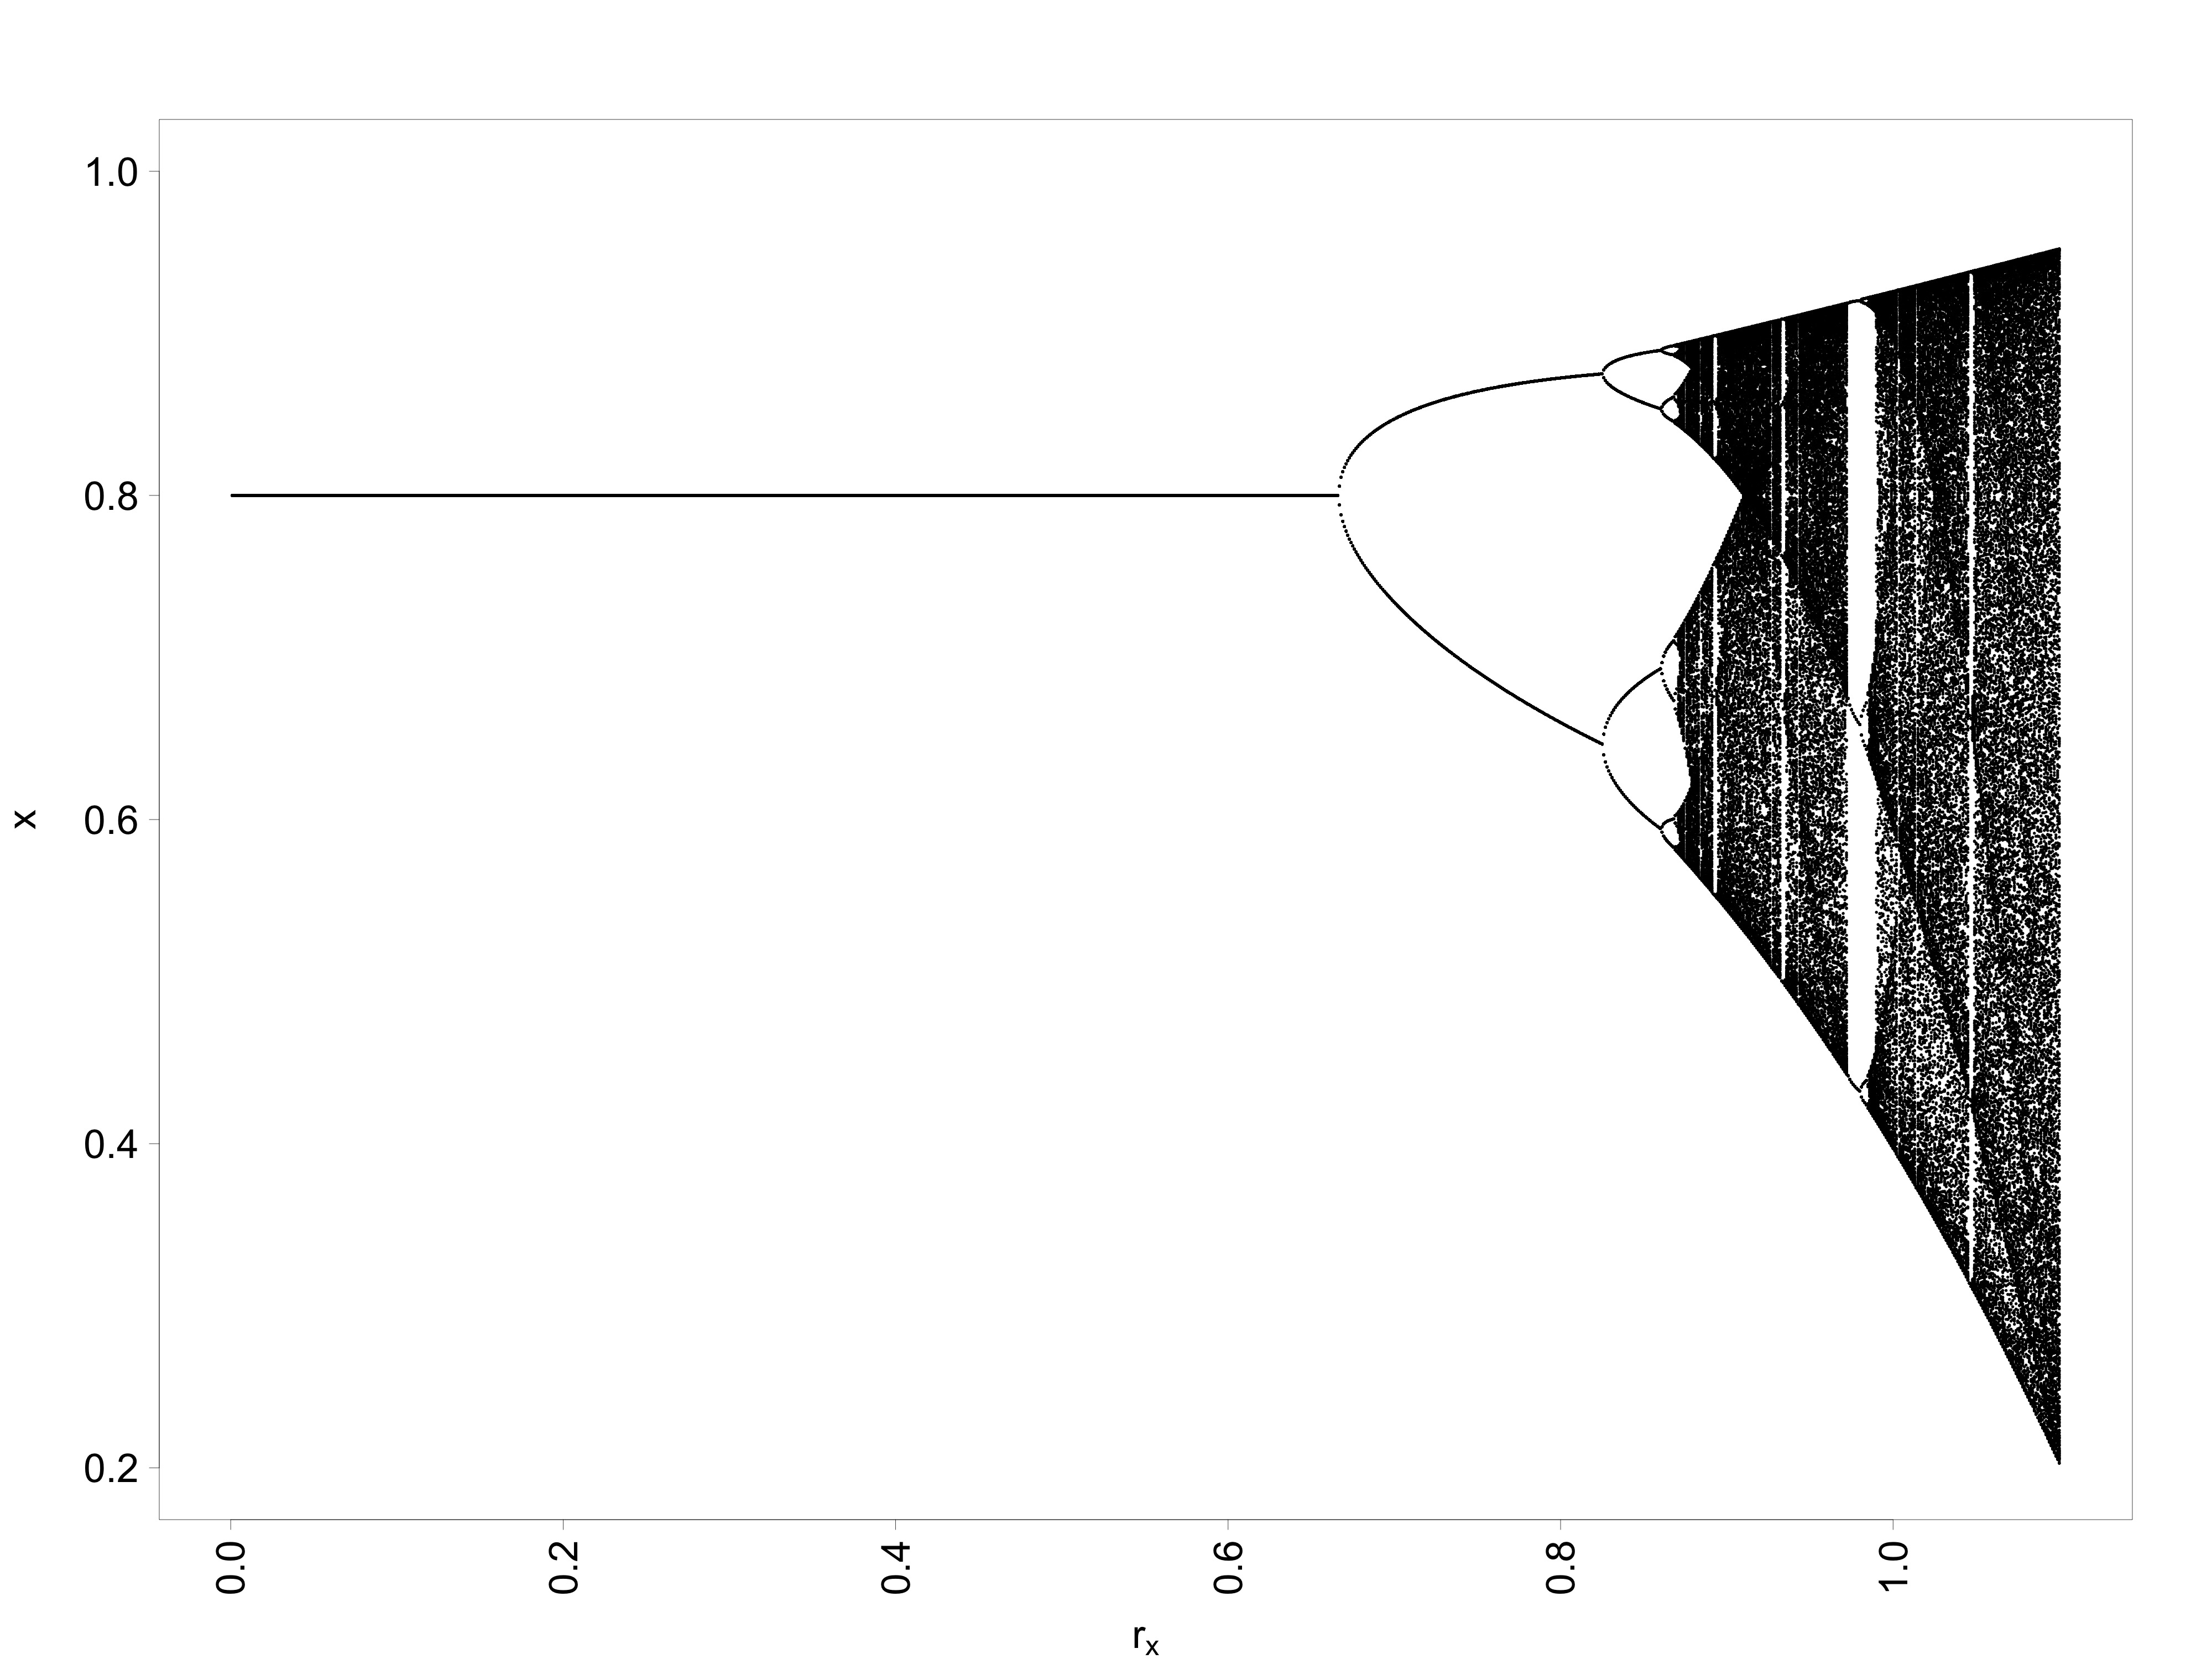
\includegraphics[width=0.7\textwidth]{./figures/figure1.jpg}
  \caption{Bifurcation diagram of a single population model with $A_x=0.2$ and $K_x=0.8$. For $0<r_x<0.6649747$, any initial value of $x$ greater than $A_x$ converge to $K_x$.}
    \label{fig:bifurcationDiagram}
\end{figure}

Here we consider only scenarios where the node $x=K_x$ is stable. In this case the initial value of $x(t=0)$ will determine the ultimate equilibria of the system: extinction, if $x(t=0)<A_x$; unstable equilibria, if $x(t=0)=A_x$; and stable equilibrium, if $x(t=0)>A_x$. Thus in a 2-trait model, the coexistence of both variants is guaranteed only when the initial density of both traits are above their respective Allee threshold, otherwise we should expect that either (i.e. $a(t=0) \geq A_a$ and $b(t=0)<A_b$ or $a(t=0)<A_a$ and $b(t=0) \geq A_b$) or both (i.e. when $a(t=0)<A_a$ and $b(t=0)<A_b$) variants will be ultimately extinct (see fig. \ref{fig:NoTransmissionBasin}). 

\begin{figure}[h!]
  \centering
      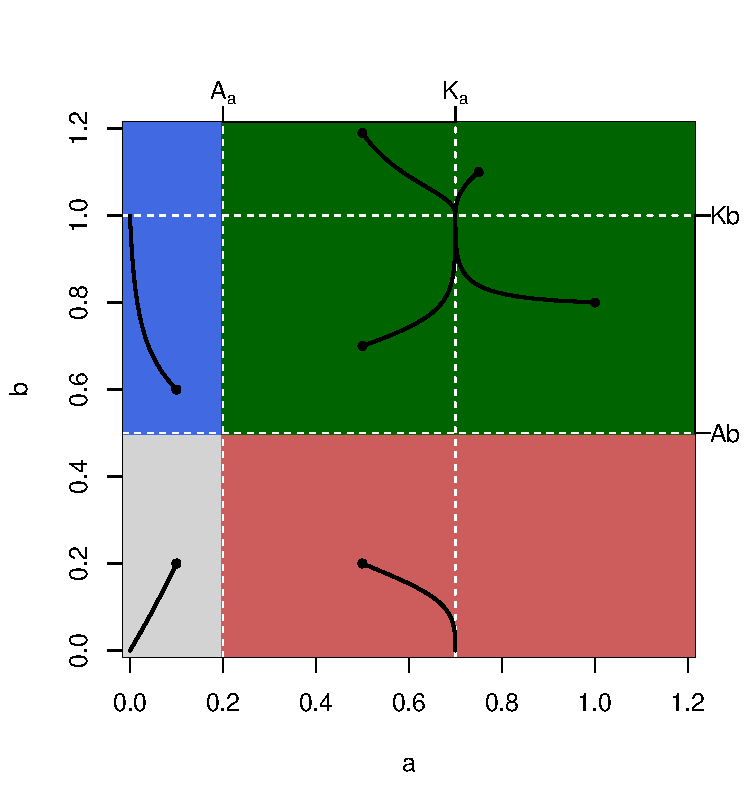
\includegraphics[width=0.7\textwidth]{./figures/figure2.pdf}
  \caption{Basins of attraction for the four equilibria (mutual extinction: grey; extinction of $a$: blue; extinction of $b$: red; stable coexistence: green). Solid lines represent trajectories of the system for different initial conditions, represented by dots. Model parameters: $A_a=0.2$; $K_a=0.7$; $A_b=0.5$; $K_b=1.0$; $r_a=r_b=0.05$}.
    \label{fig:NoTransmissionBasin}
\end{figure}

\subsection{Effects of social learning}

When social learning is enabled (i.e. when $z>0$), the stability of the nodes are perturbed by individuals switching from one strategy to another. The minimum implication of these perturbations is a change in the shape of the basins of attractions. Initial conditions closer to the boundaries between one basin and another will most profoundly be affected, potentially leading to a complete different equilibria with slightest change in the degree of reliance on social learning. Figure \ref{fig:TransmissionBasin} shows an example of this. When social learning is not present (fig.~\ref{fig:TransmissionBasin}a), the initial conditions $i$, $j$, and $k$ result into a stable equilibrium at $a=K_a$ and $b=K_b$, whilst the starting point $l$ leads to the extinction of $b$. When $z=0.05$ (fig.~\ref{fig:TransmissionBasin}b), the basins of attractions are modified, resulting into different trajectories and possibly equilibria for the same initial conditions without social learning. Thus $i$ and $k$ are no longer leading to the coexistence of both traits but to the demise of one or the other, whilst $l$ now ensure the coexistence of both variants. 

\begin{figure}[h!]
  \centering
      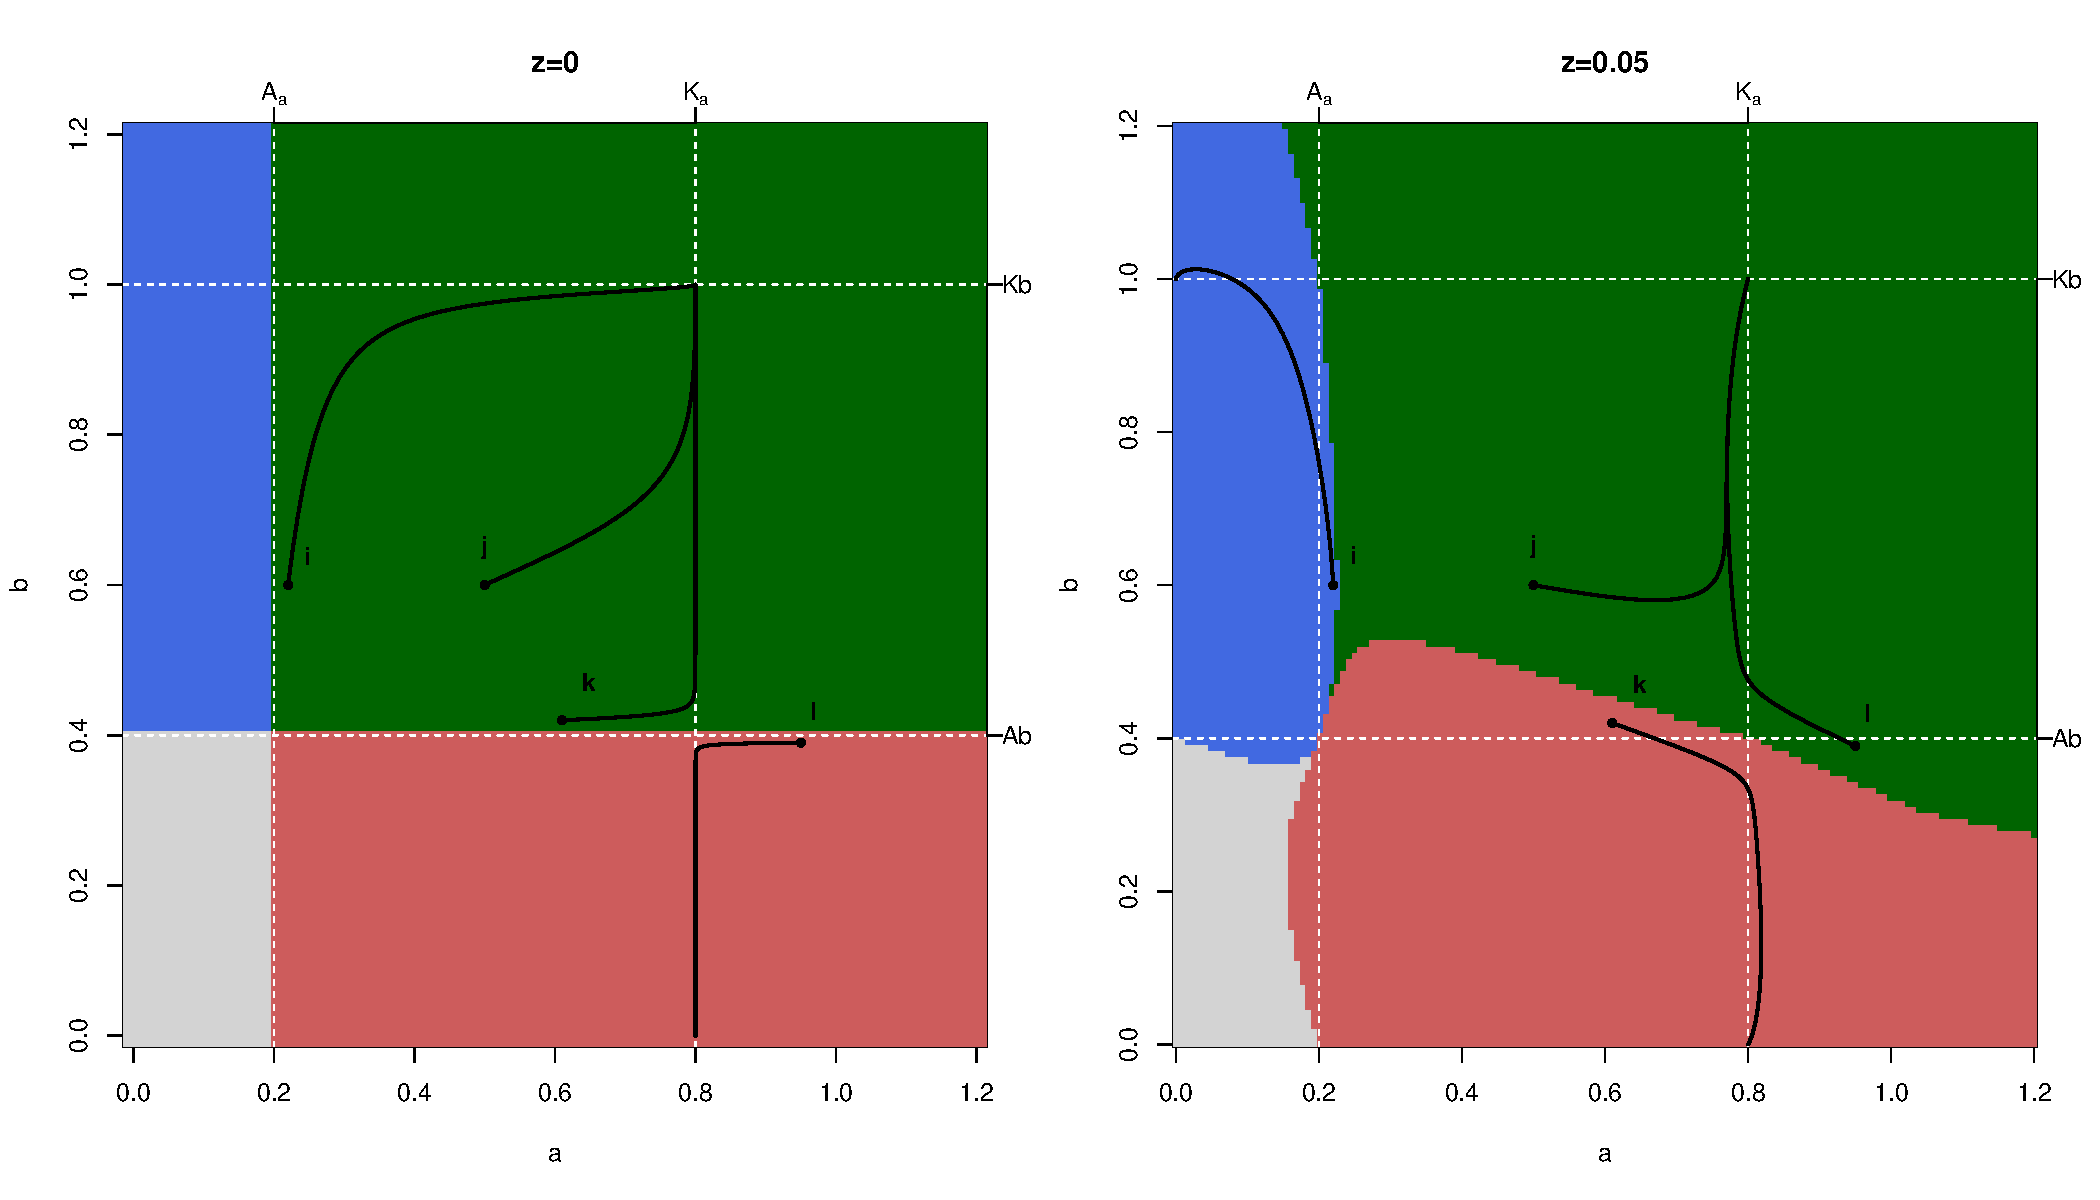
\includegraphics[width=\textwidth]{./figures/figure3.pdf}
  \caption{Basins of attraction for the four equilibria (mutual extinction: grey; extinction of $a$: blue; extinction of $b$: red; stable coexistence: green) with (right) and without (left) social learning. Model parameters: $A_a=0.2$; $K_a=0.8$; $A_b=0.4$; $K_b=1.0$; $r_a=r_b=0.05$; $z=0$ (left panel) and $z=0.05$ (right panel) }
    \label{fig:TransmissionBasin}
\end{figure}

When the magnitude of social learning is sufficiently high, the system is subject to effects similar to an increase in the per capita growth rate $r$, with the consequent decrease in the stability of the fixed points. Figure \ref{fig:bifurcationWithTransmission} shows the bifurcation diagram for three different initial settings of $a$ and $b$. In the first two cases, increase in $z$ leads to a shift of the equilibria, that remains however constant for larger reliance on social learning. The third case shows, around $z=0.5$ a transition from a point attractor to a system characterised by repeated shifts between the two transmission strategies. 
% XAVI shall we generate the pdf here?
\begin{figure}[h!]
  \centering
      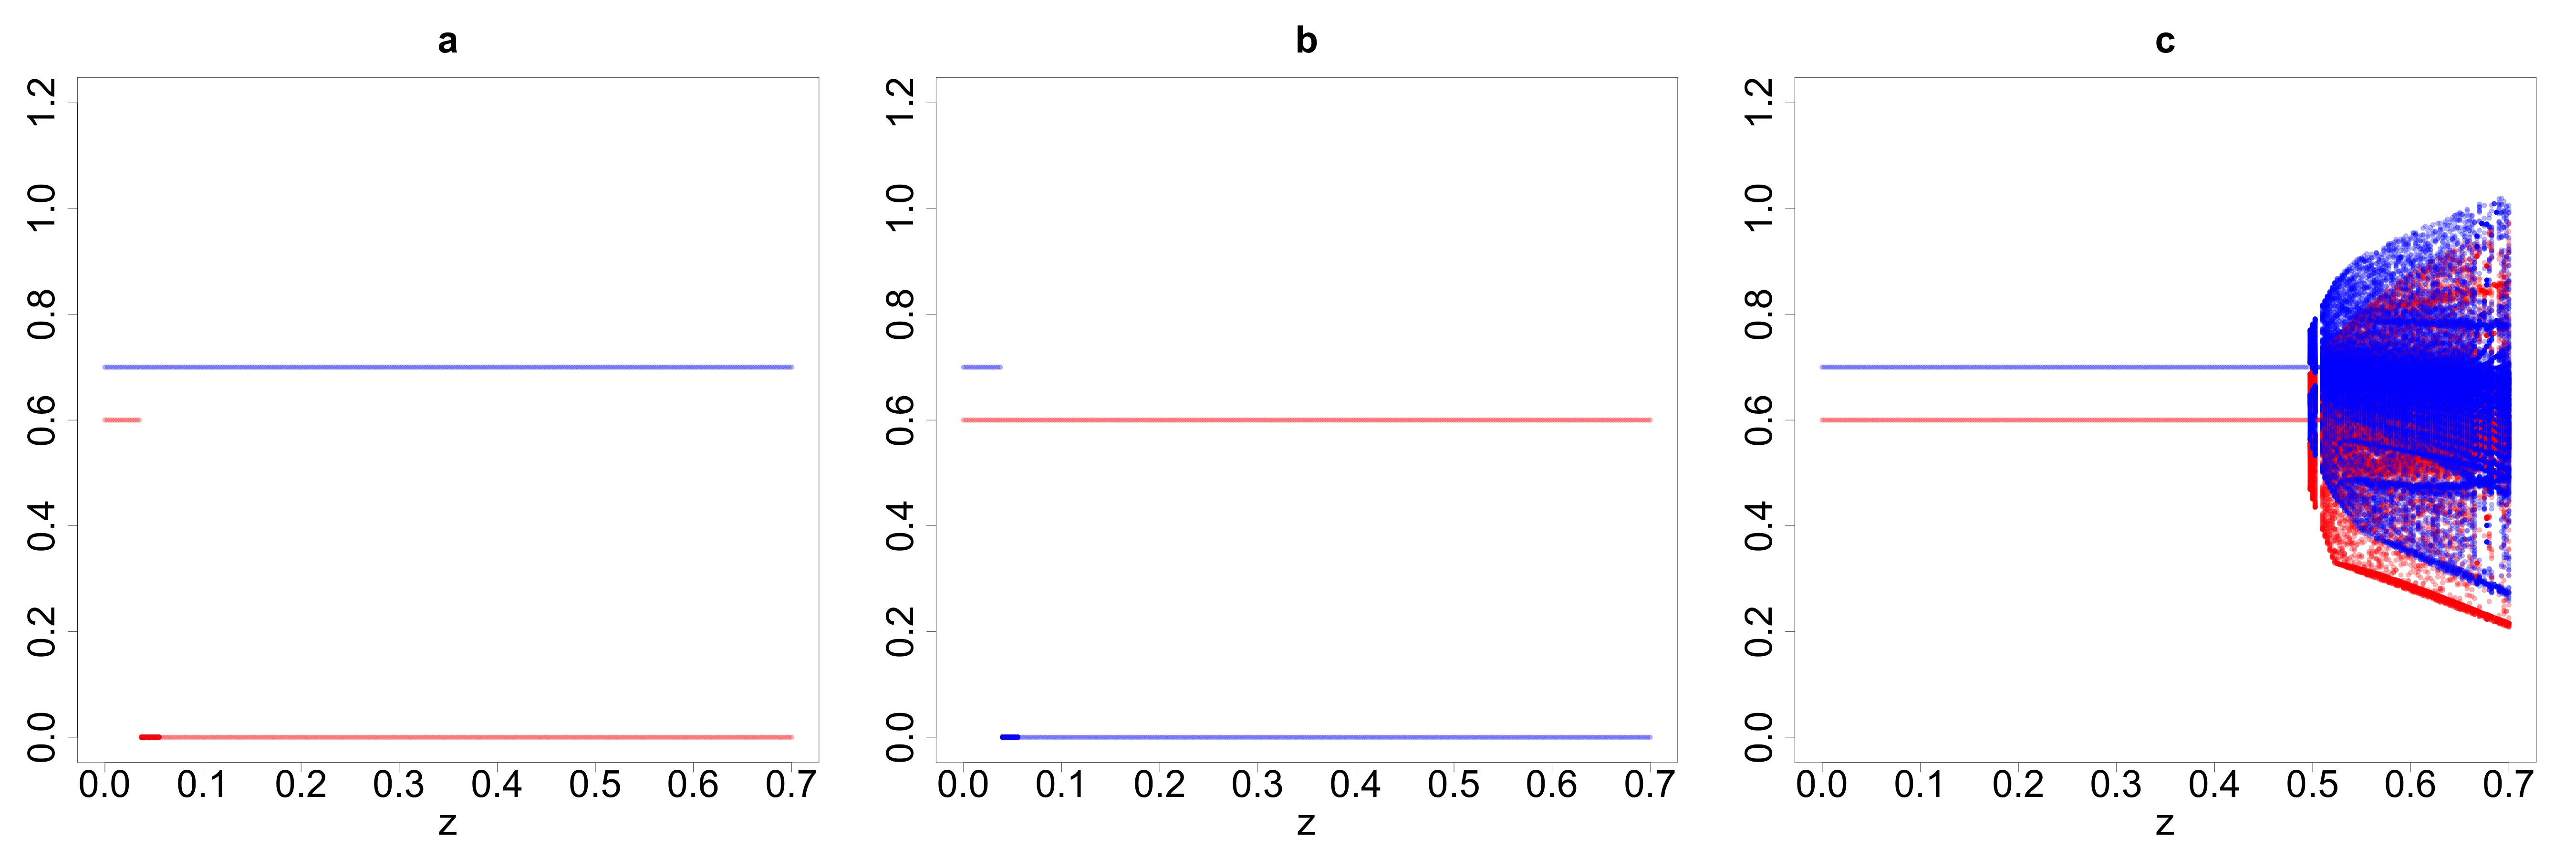
\includegraphics[width=\textwidth]{./figures/figure4.jpg}
  \caption{Bifurcation diagram for $a$ (red) and $b$ (blue) as a function of social learning ($z$): left: $a=0.11$, $b=0.4$; Middle: $a=0.5$, $b=0.21$, $a=0.4$, $b=0.4$. Model parameters:  $A_a=0.1$; $K_a=0.6$; $A_b=0.2$; $K_b=0.7$; $r_a=r_b=0.05$}
    \label{fig:bifurcationWithTransmission}
\end{figure}


\subsection{Effects of strategy overlap}
% XAVI better title?

Previous results suggest that the percentage of population that can switch strategies (i.e. the $z$ parameter) has major effects on the final equilibria. However, this will also depend on the interaction between the intervals where frequency dependence is $\geq 0$ (i.e. $[A_a,K_a]$ and $[A_b,K_b]$) . We have explored this relation introducing a new parameter $\lambda \in (0,1)$ and defining the positive interval for strategy $b$ as follows:

\begin{align}
\label{eqOverlap}
\begin{cases}
A_b = A_a + \lambda A_a\\
K_b = K_a + \lambda K_a
\end{cases}
\end{align}

The dynamics of two strategies are similar for low values of $\lambda$. High values indicate that the minimum number of individuals needed to achive positive fitness in $b$ gets closer to $K_a$, while the population size that $b$ can sustain also grows. As a consequence, the number of individuals switching strategies when $b$ has lower payoff is also higher and could potentially overload $a$ due to its lower $K_a$.

Figure XX shows how the increase in $\lambda$ affects the equilibria of our model.

% XAVI add results and figure

\subsection{Effect of competition}
%what if competition
%show new stable points
%show dynamics? 

The model described in equations \ref{eq1}-\ref{eq4} assumes that the resource pool of the two strategy are completely independent to each other. In reality many strategies have some degree of competition, whereby the frequency dependence is not exclusively internal. In other words, the frequency of one trait might increase or decrease the fitness of the other. The following equation can substitute equation~\eqref{eqCompetition}: 

\begin{align}
\begin{cases}
R_{a,t}& = r_a (\frac{a_t-c_{A_a}b_t}{A_a}-1)(1-\frac{a_t-c_{K_a}b_t}{K_a})\\
R_{b,t}& = r_b (\frac{b_t-c_{A_b}a_t}{A_b}-1)(1-\frac{b_t-c_{K_b}a_t}{K_b}) 
\end{cases}
\label{eqCompetition}
\end{align}

where the four new parameters $c_{A_a}$, $c_{A_b}$, $c_{K_a}$ and $c_{K_b}$, measure respectively the negative (or positive) effect determined by the number of individuals of the “other” traits. When $c_{A}>0$ the Allee threshold is essentially increased, while when $c_{K}>0$ the carrying capacity is diminished as function of the other population. Larger values of any of the $c$ parameters dictates a stronger influence of the other population. 

Figure XX shows a scenario where strategy $a$ is dominant over strategy $b$.
% XAVI add results and figure

\section{Discussion}


%Mention that we need more empirical evidence of Allee effect


%General Intro on Human History%
Major transitions in human history have been marked by the fast spread of key innovations, which laid the foundations of further cumulative development in economy, society, and culture. Shifts in subsistence economy has often been regarded as a prime example of these transitions, triggered by the spread of a suite of behavioural traits such as the know-how of the domestication process~\citep{barker2006} the use of new subsistence tools~\citep{petraglia_population_2009} and processing techniques~\citep{molleson1993}, and the inclusion/exclusion and extensification/intensification of different prey species %citation needed.
Archaeological evidence does not support a simple progressive adoption of these key cultural variants, and instead a showcase a variety of trajectories, including the long-term coexistence of multiple subsistence strategies, or even reversions to older traits~\citep{rowley2001}.  
  %add long list of citations. or perhaps one or two concrete examples (probably better)
\enrico{General Intro on HBE? Not sure if needed for TPB? Maybe move to discussion?}
Formal models portraying changes in human subsistence have been mostly offered in human behavioral ecology~\citep{smith1992,bird2006,kennett2006}, where several mathematical models inspired from evolutionary ecology %we need a better one-line description of HBE. 
 used to predict  based on expected patterns under the assumption of optimality~\citep{belovsky1988}. 
While earliest models relied almost exclusively on this assumption, most recent works are increasing discussing how the knowledge of alternative subsistence strategies are acquired %citation needed? Are there such works? Need to check
and whether this process of learning can drive the evolutionary trajectory of a given population~\citep{henrich1998}, partly as a synergy with the dual inheritance theory~\citep{boyd1985}. 

The results of these works often exhibits counter-intuitive outcomes that cannot be predicted by standard assumptions of optimality. For instance, extreme reliance on social learning can promote information parasitism~\citep{giraldeau2002}, leading to a decline in the proportion of asocial learners that in certain environmental context can have strongly detrimental effects at the population level~\citep{whitehead2009}. Other examples include instances where a reduced effective population size promotes an increase in random drift, and the ultimate loss of adaptive traits~\citep{henrich2004}, or instances where neutral traits are jointly transmitted together with adaptive ones~\citep{ackland2007}. These examples illustrate how theoretical models based on the dual inheritance theory can extend predictions of the standard optimal foraging theory, integrating dynamics that, at least at a first glance, are regarded as counter-intuitive. 

These include episodes of reversions (e.g. \footnote{citation needed}), where a more recent optimal strategies are abandoned for older suboptimal variants; stable coexistence (e.g. \footnote{citation needed}), where optimal and suboptimal strategies co-exist within a population; and even the complete loss of optimal variants~\citep[e.g.][]{henrich2004}. The evolutionary processes leading to these different outcomes are undoubtedly contingent to local historical dynamics, nonetheless we argue that a simple model of social learning in combination with a positive and negative frequency dependent selection can lead all these equilibria.


\enrico{We need to mention that some behaviour might actually enhance the other community (or be detrimental). This can be modelled using a competition coefficient as in~\citep{jang2013}. I don't think we need to explore this but it is definitely worth mentioning!}

\enrico{Mutually exclusive trait, but does not necessarily imply HG vs FA mixture of strategy (say 50\%HG vs 50\%F) can be assumed to be a trait. Perhaps this needs to be mentioned earlier when the model is introduced.}


\section{References}

\bibliographystyle{elsarticle-harv}
\bibliography{references}

\section{Appendix I}

-50,000 iterations
-floating point arithmetic



\end{document}

